\fakesection{Probabilistic Inference Using Weighted Model Counting}

%%%
%%%
%%%

\fakesubsection{SRL to CNF}

First the program is grounded. This is a matter of collecting all atoms involved in all proofs of the query.

\begin{code}
\begin{minted}[xleftmargin=20pt,linenos]{PROLOG}
0.2::stress(a).
0.2::stress(b).
0.2::stress(c).

0.1::friends(a,a).
0.1::friends(a,b).
0.1::friends(a,c).

0.1::friends(b,a).
0.1::friends(b,b).
0.1::friends(b,c).

0.1::friends(c,a).
0.1::friends(c,b).
0.1::friends(c,c).

0.3::smokes(a) :- stress(a).
0.3::smokes(b) :- stress(b).
0.3::smokes(c) :- stress(c).

0.4::smokes(a) :- friends(a,a), smokes(a).
0.4::smokes(a) :- friends(a,b), smokes(b).
0.4::smokes(a) :- friends(a,c), smokes(c).
0.4::smokes(b) :- friends(b,a), smokes(a).
0.4::smokes(b) :- friends(b,b), smokes(b).
0.4::smokes(b) :- friends(b,c), smokes(c).

0.4::smokes(c) :- friends(c,a), smokes(a).
0.4::smokes(c) :- friends(c,b), smokes(b).
0.4::smokes(c) :- friends(c,c), smokes(c).
\end{minted}
\captionof{listing}{Relevant ground program.}
\label{code:base}
\vspace{0.5cm}
\end{code}

\definecolor{darkgray}{rgb}{0.4,0.4,0.4}
\definecolor{c1}{rgb}{0.83,0.13,0.18}
\definecolor{c2}{rgb}{0.23,0.48,0.34}
\definecolor{c3}{rgb}{0.18,0.35,0.58}
\begin{figure*}[h]
\centering
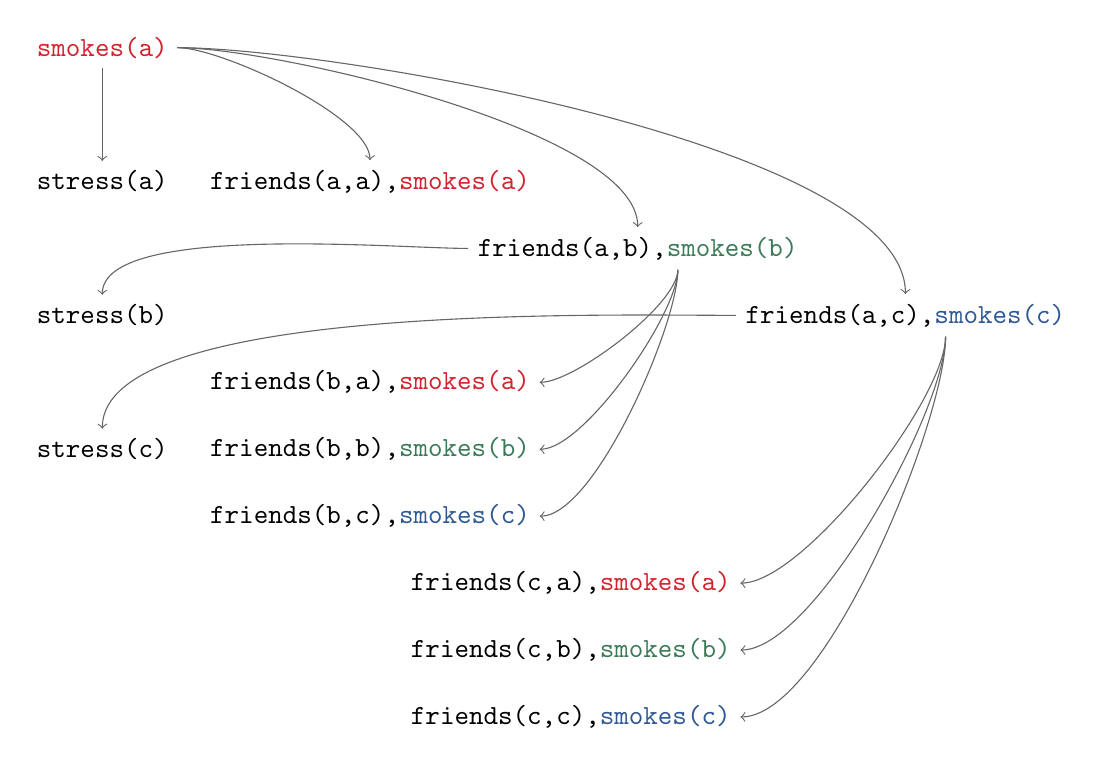
\begin{tikzpicture}[scale=0.85]

	\node at (0,0) (1) {\texttt{\textcolor{c1}{smokes(a)}}};
	
	\node at (0,-2) (2) {\texttt{stress(a)}};
	\node at (0,-4) (6) {\texttt{stress(b)}};
	\node at (0,-6) (7) {\texttt{stress(c)}};
	
	\node at (4,-2) (3) {\texttt{friends(a,a),\textcolor{c1}{smokes(a)}}};
	\node at (8,-3) (4) {\texttt{friends(a,b),\textcolor{c2}{smokes(b)}}};
	\node at (12,-4) (5) {\texttt{friends(a,c),\textcolor{c3}{smokes(c)}}};
	
	\node at (4,-5) (8) {\texttt{friends(b,a),\textcolor{c1}{smokes(a)}}};
	\node at (4,-6) (9) {\texttt{friends(b,b),\textcolor{c2}{smokes(b)}}};
	\node at (4,-7) (10) {\texttt{friends(b,c),\textcolor{c3}{smokes(c)}}};
	
	\node at (7,-8) (11) {\texttt{friends(c,a),\textcolor{c1}{smokes(a)}}};
	\node at (7,-9) (12) {\texttt{friends(c,b),\textcolor{c2}{smokes(b)}}};
	\node at (7,-10) (13) {\texttt{friends(c,c),\textcolor{c3}{smokes(c)}}};
	
	\draw[darkgray,->] (1.south) to (2.north);
	
	\draw[darkgray,->] (1.east) to [out=0,in=90,looseness=0.5](3.north);
	\draw[darkgray,->] (1.east) to [out=0,in=90,looseness=0.5](4.north);
	\draw[darkgray,->] (1.east) to [out=0,in=90,looseness=0.5](5.north);
	
	\draw[darkgray,->] (4.west) to [out=180,in=90,looseness=0.5](6.north);
	\draw[darkgray,->] (5.west) to [out=180,in=90,looseness=0.5](7.north);
	
	\draw[darkgray,->] ([xshift=6mm]4.south) to [out=-90,in=0,looseness=0.5](8.east);
	\draw[darkgray,->] ([xshift=6mm]4.south) to [out=-90,in=0,looseness=0.5](9.east);
	\draw[darkgray,->] ([xshift=6mm]4.south) to [out=-90,in=0,looseness=0.5](10.east);
	
	\draw[darkgray,->] ([xshift=6mm]5.south) to [out=-90,in=0,looseness=0.5](11.east);
	\draw[darkgray,->] ([xshift=6mm]5.south) to [out=-90,in=0,looseness=0.5](12.east);
	\draw[darkgray,->] ([xshift=6mm]5.south) to [out=-90,in=0,looseness=0.5](13.east);
	
	% Loops
	
	%\draw[->,dashed,blue] ([xshift=-4mm]3.north) to ([xshift=4mm]1.south);
%	
%	\draw[->,dashed,blue] ([xshift=-4mm]8.north) to ([xshift=4mm,looseness=0.5]1.south);
%	\draw[->,dashed,blue] ([xshift=-4mm]9.east) to ([xshift=4mm,looseness=0.5]4.south);
%	\draw[->,dashed,blue] ([xshift=-4mm]10.east) to ([xshift=4mm,looseness=0.5]5.south);
%	
%	\draw[->,dashed,blue] ([xshift=-4mm]11.east) to ([xshift=4mm,looseness=0.5]1.south);
%	\draw[->,dashed,blue] ([xshift=-4mm]12.east) to ([xshift=4mm,looseness=0.5]4.south);
%	\draw[->,dashed,blue] ([xshift=-4mm]13.east) to ([xshift=4mm,looseness=0.5]5.south);
	
%	\node at (-2.5,5) (3) {$\mathbb{N}$};
%	\draw[->,shorten >=1pt] (3) to [out=180,in=-90,loop,looseness=15] node[left]{$id$} (3);
%	\draw[->,shorten >=1pt] (3) to [out=180,in=-90,loop,looseness=30] node[left]{$add1mod3$} (3);
%	\draw[->,shorten >=1pt] (3) to [out=180,in=-90,loop,looseness=45] node[left]{$add2mod3$} (3);
\end{tikzpicture}
\caption{SLG-tree produced while turning the ground program into a boolean formula. Coloured atoms indicate the presence of cycles.}
\label{fig:nestedtries}
\end{figure*}

\noindent The proofs of the query make for a trie as shown in figure \ref{fig:nestedtries}, where colourings indicate the presence of cycles. Any proof involving an atom \texttt{friends(X,X)} or \texttt{friends(Y,a)} (with $Y\in\{b,c\}$) is non-minimal and doesn't affect the final probability. These atoms are disregarded. For the remaining cycles (involving \texttt{friends(b,c)} and \texttt{friends(c,b)}) auxiliary variables can be used to obtain a cycle-free program :

\begin{code}
\begin{minted}[xleftmargin=20pt,linenos]{PROLOG}
0.2::stress(a).
0.2::stress(b).
0.2::stress(c).

0.1::friends(a,b).
0.1::friends(a,c).
0.1::friends(b,c).
0.1::friends(c,b).

0.3::p(a).
0.3::p(b).
0.3::p(c).

0.4::p(a,b).
0.4::p(a,c).
0.4::p(b,c).
0.4::p(c,b).

smokes(a) :- stress(a), p(a).
smokes(b) :- stress(b), p(b).
smokes(c) :- stress(c), p(c).

smokes(a) :- 
    friends(a,b), smokes(b), p(a,b).
smokes(a) :-
    friends(a,c), smokes(c), p(a,c).
smokes(b) :- 
    friends(b,c), stress(c), p(c), p(b,c).
smokes(c) :- 
    friends(c,b), stress(b), p(b), p(c,b).

query(smokes(a)).
\end{minted}
\captionof{listing}{Relevant ground program without cycles.}
\label{code:base}
\vspace{0.5cm}
\end{code}

\noindent The above logic program is equivalent to the following propositional formula :
\begin{center}
\begin{tabular}{ll}
$(smokes(a)\leftrightarrow$ & $(stress(a) \land p(a))$\\
\multicolumn{2}{c}{$\lor\ (friends(a,b) \land smokes(b) \land p(a,b))$}\\
\multicolumn{2}{c}{$\lor\ (friends(a,c) \land smokes(c) \land p(a,c)))$}\\
\multicolumn{2}{c}{$\land$}\\
$(smokes(b)\leftrightarrow$ & $(stress(b) \land p(b))$\\
\multicolumn{2}{c}{$\lor\ (friends(b,c) \land stress(c) \land p(c) \land p(b,c)))$}\\
\multicolumn{2}{c}{$\land$}\\
$(smokes(c)\leftrightarrow$ & $(stress(c) \land p(c))$\\
\multicolumn{2}{c}{$\lor\ (friends(c,b) \land stress(b) \land p(b) \land p(c,b)))$}\\
\end{tabular}
\end{center}

\vspace{0.1cm}
\par\noindent Which gives the following \texttt{CNF} :\vspace{0.3cm}\\
$(\lnot smokes(a) \lor stress(a) \lor friends(a,b) \lor friends(a,c))
\\\land (\lnot smokes(a) \lor stress(a) \lor friends(a,b) \lor smokes(c))
\\\land (\lnot smokes(a) \lor stress(a) \lor smokes(b) \lor friends(a,c))
\\\land (\lnot smokes(a) \lor stress(a) \lor smokes(b) \lor smokes(c))
\\\land (\lnot stress(a) \lor smokes(a))
\\\land (\lnot friends(a,b) \lor \lnot smokes(b) \lor smokes(a))
\\\land (\lnot friends(a,c) \lor \lnot smokes(c) \lor smokes(a))
\\\land (\lnot smokes(b) \lor p(b) \lor friends(b,c))
\\\land (\lnot smokes(b) \lor p(b) \lor p(c))
\\\land (\lnot p(b) \lor smokes(b))
\\\land (\lnot friends(b,c) \lor \lnot p(c) \lor smokes(b))
\\\land (\lnot smokes(c) \lor p(c) \lor friends(c,b))
\\\land (\lnot smokes(c) \lor p(c) \lor p(b))
\\\land (\lnot p(c) \lor smokes(c))
\\\land (\lnot friends(c,b) \lor \lnot p(b) \lor smokes(c))
\\\land (\lnot p(b) \lor stress(b)) 
\\\land (\lnot stress(b) \lor p(b)) 
\\\land (\lnot p(c) \lor stress(c)) 
\\\land (\lnot stress(c) \lor p(c))$
\vspace{0.3cm}

\par\noindent The probabilistic literals \texttt{CNF} are assigned weights (derived literals have a weight of 1) :

\begin{center}
\begin{tabular}{c|c}
Atom & Weight \\
\hline
stress(a) & 0.2 \\
$\lnot$stress(a) & 0.8 \\
stress(b) & 0.2 \\
$\lnot$stress(b) & 0.8 \\
stress(c) & 0.2 \\
$\lnot$stress(c) & 0.8 \\
friends(a,b) & 0.1 \\
$\lnot$friends(a,b) & 0.9 \\
friends(a,c) & 0.1 \\
$\lnot$friends(a,c) & 0.9 \\
friends(b,c) & 0.1 \\
$\lnot$friends(b,c) & 0.9 \\
friends(c,b) & 0.1 \\
$\lnot$friends(c,b) & 0.9 \\
\end{tabular}
\end{center}

%%%
%%%
%%%

\fakesubsection{SRL to PGM}



%%%
%%%
%%%

\fakesubsection{PGM to CNF}



%%%
%%%
%%%

\fakesubsection{Weighted Model Counting}